\fontfamily{\sfdefault}\selectfont
% XCircuit output "direct_type_1.tex" for LaTeX input from direct_type_1.ps
\def\putbox#1#2#3#4{\makebox[0.00000in][l]{\makebox[#1][l]{}\raisebox{\baselineskip}[0.00000in][0.00000in]{\raisebox{#2}[0.00000in][0.00000in]{\scalebox{#3}{#4}}}}}
\def\rightbox#1{\makebox[0.00000in][r]{#1}}
\def\centbox#1{\makebox[0.00000in]{#1}}
\def\topbox#1{\raisebox{-0.60\baselineskip}[0.00000in][0.00000in]{#1}}
\def\midbox#1{\raisebox{-0.20\baselineskip}[0.00000in][0.00000in]{#1}}
   \scalebox{1}{
   \normalsize
   \parbox{2.59948in}{
   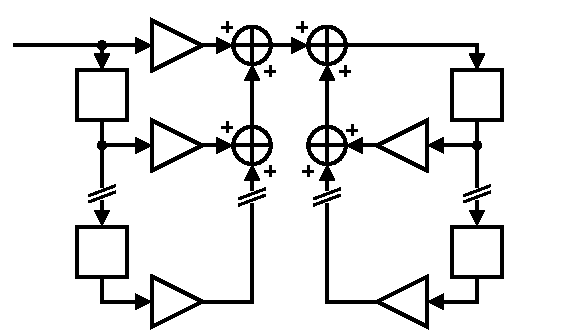
\includegraphics[scale=0.70000]{./figs/direct_type_1.pdf}\\
   % translate x=936 y=992 scale 0.38
   \putbox{0.04200in}{1.42800in}{0.96}{x[n]}%
   \putbox{2.28200in}{1.33700in}{0.96}{y[n]}%
   \putbox{0.37800in}{1.07800in}{0.96}{$z^{-1}$}%
   \putbox{0.84000in}{1.45600in}{0.96}{b$_0$}%
   \putbox{0.84000in}{0.98700in}{0.96}{b$_1$}%
   \putbox{2.12800in}{1.07800in}{0.96}{$z^{-1}$}%
   \putbox{2.12800in}{0.34300in}{0.96}{$z^{-1}$}%
   \putbox{1.71500in}{1.00100in}{0.96}{-a$_1$}%
   \putbox{1.70100in}{0.27300in}{0.96}{-a$_\mathrm{P}$}%
   \putbox{2.28200in}{0.86800in}{0.96}{y[n-1]}%
   \putbox{0.37800in}{0.34300in}{0.96}{$z^{-1}$}%
   \putbox{0.84000in}{0.25900in}{0.96}{b$_\mathrm{Z}$}%
   } % close 'parbox'
   } % close 'scalebox'
   \vspace{-\baselineskip} % this is not necessary, but looks better
\fontfamily{\rmdefault}\selectfont
